\newcommand{\department}{САПР}
% \newcommand{\labnum}{0}
\newcommand{\discipline}{Программирование}
\newcommand{\theme}{Разработка электронной картотеки}
\newcommand{\haspartner}{1}
\newcommand{\partnername}{Миллер В.В.}
\newcommand{\teachername}{Кузьмин С.А.}
\newcommand{\labyear}{2020}

\documentclass[12pt,a4paper]{article}  % шаблон для статьи, шрифт 12 пт

\usepackage[utf8]{inputenc}  % использование кодировки Юникод UTF-8

\usepackage[T1]{fontenc}

\usepackage[russian]{babel}  % пакет поддержки русского языка

\usepackage{graphicx}  % кртинки

\usepackage[labelsep=endash]{caption}  % тире вместо двоеточия в картинках

\usepackage{indentfirst}  % отступ первого абзаца
\setlength{\parindent}{0.75cm}

\usepackage[compact]{titlesec}  % для titlespacing
% \titlespacing{\заголовок}{слева}{перед}{после}[справа]
\titlespacing*{\section}{0.75cm}{1em}{0.1em}  % отступ заголовка
\titlespacing*{\subsection}{0.75cm}{1em}{0.1em}


\usepackage{xcolor}
\usepackage{listings}  % листинги кода из файлов

\definecolor{codegreen}{rgb}{0,0.6,0}
\definecolor{codegray}{rgb}{0.5,0.5,0.5}
\definecolor{codepurple}{rgb}{0.58,0,0.82}
\definecolor{backcolour}{rgb}{0.95,0.95,0.92}

\lstdefinestyle{cpp}
{
	backgroundcolor=\color{backcolour},% цвет фона подсветки
	commentstyle=\color{codegreen},
	keywordstyle=\color{magenta},
	numberstyle=\small\color{codegray},% размер шрифта для номеров строк
	stringstyle=\color{codepurple},
	basicstyle=\ttfamily\footnotesize, % размер и начертание шрифта для подсветки кода
	breakatwhitespace=false,           % переносить строки только если есть пробел  
	breaklines=true,                   % автоматически переносить строки (да\нет)  
	captionpos=t,                      % позиция заголовка вверху [t] или внизу [b]
	keepspaces=true,                 
	numbers=left,                   % где поставить нумерацию строк (слева\справа)            
	numbersep=5pt,                  % как далеко отстоят номера строк от подсвечиваемого кода           
	showspaces=false,               % показывать или нет пробелы специальными отступами       
	showstringspaces=false,         % показывать или нет пробелы в строках
	showtabs=false,                 % показывать или нет табуляцию в строках        
	tabsize=2,                      % размер табуляции по умолчанию равен 2 пробелам
	language=c++,                   % выбор языка для подсветки (здесь это С++)                   
	stepnumber=1,                   % размер шага между двумя номерами строк
	frame=false,                    % рисовать рамку вокруг кода
	escapeinside={\%*}{*)},         % если нужно добавить комментарии в коде
	extendedchars=\true
}

\lstset{style=cpp}
\usepackage{graphicx}  % кртинки
\usepackage{float} % плавающие картинки
\usepackage{wrapfig}  % Обтекание фигур (таблиц, картинок и прочего)
\usepackage[labelsep=endash]{caption}  % тире вместо двоеточия в картинках
\renewcommand\thefigure{\arabic{section}.\arabic{figure}}
\usepackage{tabularx}




\begin{document}

	\thispagestyle{empty}

\begin{center}
    \Large{
    \textbf{МИНОБРНАУКИ РОССИИ}

    \textbf{Санкт-Петербургский государственный}

    \textbf{электротехнический университет «ЛЭТИ»}

    \textbf{им. В.И. Ульянова (Ленина)}

    \textbf{Кафедра \department}
    }
\end{center}

\topskip=0pt
\vspace*{\fill}

\begin{center}
    \Large{
    \textbf{
    КУРСОВАЯ РАБОТА\\
    по дисциплине «\discipline»\\
    Тема: \theme\\
    }
    }
\end{center}

\vspace*{\fill}

\begin{tabular}{lcr}
    Студенты гр. 9892 & \begin{tabular}{p{60mm}} \\ \hline \end{tabular} & Лескин К.А.  \\\\
    \if \haspartner 1
                      & \begin{tabular}{p{60mm}} \\ \hline \end{tabular} & \partnername \\\\
    \fi
    Преподаватель     & \begin{tabular}{p{60mm}} \\ \hline \end{tabular} & \teachername
    \\\\
\end{tabular}

\begin{center}
    Санкт-Петербург\\
    \labyear
\end{center}

\newpage

	\begin{center}
	\Large{
		\textbf{Задание\\ на курсовую работу}
	}
\end{center}

\textbf{Студенты:} Лескин К.А., Миллер В.В.\\

\textbf{Группа:} 9892\\

\textbf{Тема работы:} Разработка электронной картотеки\\

\textbf{Исходные данные:}

Разработать программу, позволяющую выполнять различные операции
над базой данных, представленной в виде линейного списка (тема базы
данных и набор операций есть в своём варианте задания).

Курсовая работа «собирается» студентом из функций, объединённых с
помощью меню в головной программе, выполняющей обработку связанного
линейного списка.

В виде отдельных пользовательских функций оформляются части
программы, реализующие операции:
\begin{itemize}
	\item создание списка (выделение памяти, создание и заполнение вводимыми с
	клавиатуры данными элементов списка);
	\item сохранение введённой информации в заданном пользователем файле;
	\item восстановление списка (заполнение его информацией, считываемой из
	файла, поиск элемента по признаку (признак - одно из полей структуры));
	\item сортировка найденных элементов и вывод информации о них на экран;
	\item корректировка полей записи выбранного элемента (идентификация
	элемента по номеру в выводимом на экран перечне (по номеру указателя
	на элемент));
	\item удаление выбранного элемента (одного из найденных по признаку);
	\item вставка нового элемента (после/перед выбранным).
\end{itemize}

\newpage

\textbf{Индивидуальный вариант №10}:

Обеспечить работу компании, осуществляющей грузовые
перевозки на основе наличия:

\begin{itemize}
	\item списка парка грузовиков (марка, грузоподъёмность, максимальная
	дальность перевозки, плановый пробег в пути за сутки);
	\item списка водителей (ФИО, разрешение на использование марки грузовика);
	\item списка маршрутов перевозки (конечный пункт, дальность, время
	погрузки/разгрузки в конечных пунктах, количество водителей).
\end{itemize}

При поступлении очередного заказа (маршрут, дата выезда, масса груза,
пожелание по марке грузовика) необходимо сформировать для поездки
комбинацию грузовик-водитель(-и).

Дополнительно необходимо выдавать информацию:

\begin{itemize}
	\item о свободных водителях на определённую дату;
	\item о свободных грузовиках на определённую дату;
	\item о грузовиках, находящихся на определённом маршруте;
	\item о водителях, находящихся на определённом маршруте;
	\item о плановой дате прибытия грузовика с водителем(-ями).

\end{itemize}

\newpage

\textbf{Содержание пояснительной записки:}\\
\textbf{Требуемые разделы пояснительной записки:} «Содержание», «Введение», Основные главы,
«Заключение», «Список использованных источников».\\

\textbf{Предполагаемый объем пояснительной записки:}\\
Не менее 30 страниц.\\

\textbf{Дата выдачи задания:} 29.09.2020
\\

\textbf{Дата сдачи курсовой работы:} 23.12.2020
\\

\textbf{Дата защиты курсовой работы:} 29.12.2020
\\

\begin{tabular}{lcr}
	Студенты гр. 9892 & \begin{tabular}{p{60mm}} \\ \hline \end{tabular} & Лескин К.А.  \\\\ 
	& \begin{tabular}{p{60mm}} \\ \hline \end{tabular} & Миллер В.В.  \\\\ 
	Преподаватель     & \begin{tabular}{p{60mm}} \\ \hline \end{tabular} & Кузьмин С.А. \\\\
\end{tabular}
	
	\newpage

	\begin{center}
	\Large{
		\textbf{Аннотация}
	}
\end{center}

В данной курсовой работе необходимо реализовать программу, обрабатывающую текстовые данные, хранящиеся в виде файлов, в соответствии с опцией, которую выбирает пользователь. Данные небходимо хранить в памяти компьютера в виде списка. Пользовательский интерфейс включает в себя меню, которое позволяет производить все необходимые манипуляции с исходными данными. Для выполнения данной курсовой работы будут использованы знания, полученные при выполнении лабораторных работ. В результате будет получена программа полностью соответствующая требованиям к индивидуальному заданию.
\\
\\
\\
\\
\\
\\
\\
\\
\\
\begin{center}
	\Large{
		\textbf{Summary}
	}
\end{center}

In this coursework, it is needed to implement a program that processes text data stored as files, in accordance with the option that the user chooses. Data should be stored as a list. The user interface includes a menu that allows you to make all the necessary manipulations with the original data. In this coursework we will use the knowledge gained during laboratory work. As a result, the program will be fully compliant with the requirements for the individual task.
	
	\newpage
	
	\tableofcontents
	
	\newpage
	
	\section{Введение}
%\addcontentsline{toc}{section}{Введение}

Целью данной курсовой работы является приобретение навыков разработки и отладки многомодульных
программ на языке C++. Разработка программы, позволяющей создать,
обработать, вывести и удалить базу данных на основе линейных списков.

В ходе выполнения работы мы воспользуемся всеми знаниями, полученными при выполнении лабораторных работ.
Содержание пояснительной записки к курсовой работе соответствует стандартным требованиям к пояснительным документам для программного продукта.

В данной курсовой работе предполагается использование функций для
работы с структурой данных "список" [ссылка]. 

	
	\section{Внешние форматы хранения данных}
%\addcontentsline{toc}{section}{Внешние форматы хранения данных}

Файлы для баз данных хранятся в формате CSV (Comma Separated Values) [ссылка]. В каждом файле присутствует заголовочная строка, показывающая какие данные хранятся в каждом столбце.

CSV формат так же применяется для запросов.

Для грузовиков определены следующие столбцы:
\begin{itemize}
	\item id -- идентификационный номер грузовика (int);
	\item brand -- код марки грузовика (int);
	\item capacity -- грузоподъёмность грузовика в тоннах (float);
	\item transportation\_distance -- максимальная дальность перевозки (int).
\end{itemize}

Пример таблицы грузовиков указан на рис. \ref{truck_table}.

\begin{figure}[hpt!]
	\centering
	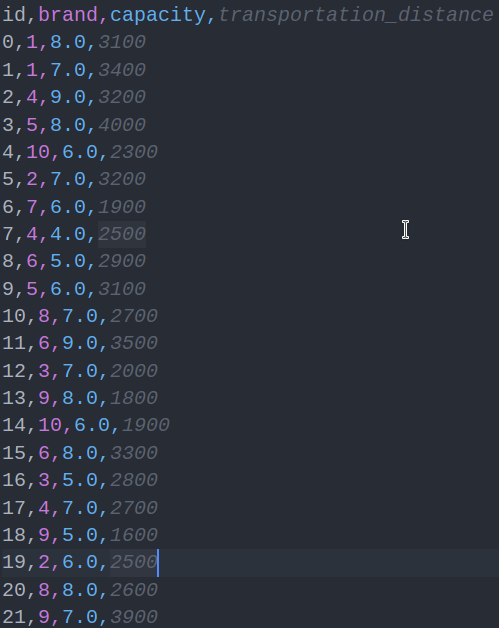
\includegraphics[width=0.5\linewidth]{photo/truck_table}
	\caption{Пример таблицы грузовиков}
	\label{truck_table}
\end{figure}

\newpage
Для водителей определены следующие столбцы:
\begin{itemize}
	\item id -- идентификационный номер водителя (int);
	\item name -- имя водятеля (string);
	\item name -- фамилия водятеля (string);
	\item name -- отчество водятеля (string);
	\item brand\_code -- код разрешённой марки грузовика (int).
\end{itemize}

Пример таблицы водителей указан на рис. \ref{driver_table}.

\begin{figure}[hpt!]
	\centering
	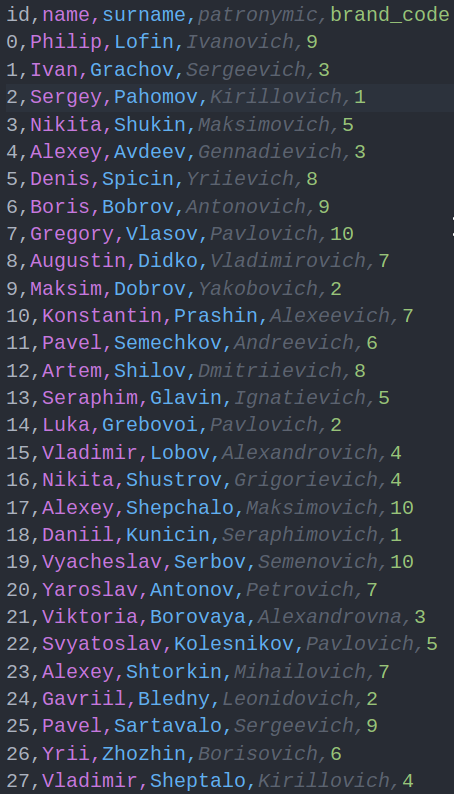
\includegraphics[width=0.5\linewidth]{photo/driver_table}
	\caption{Пример таблицы водителей}
	\label{driver_table}
\end{figure}

\newpage

Для маршрутов определены следующие столбцы:
\begin{itemize}
	\item id -- идентификационный номер маршрута (int);
	\item destination\_code -- код конечного пункта (int);
	\item distance -- длина маршрута в км (int);
	\item loading\_time -- время погрузки/разгрузки в конечных пунктах в ч (int);
	\item drivers -- кол-во водителей (int);
	\item time\_in\_transit -- расчётное время поставки в одну сторону (ч) (int).
\end{itemize}

Пример таблицы маршрутов указан на рис. \ref{route_table}.

\begin{figure}[hpt!]
	\centering
	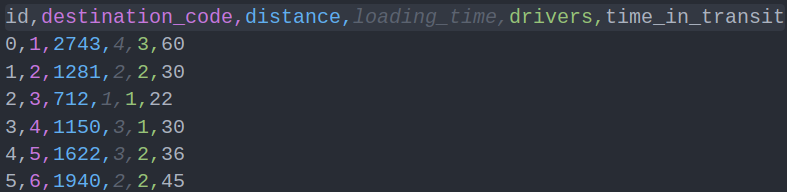
\includegraphics[width=0.8\linewidth]{photo/route_table}
	\caption{Пример таблицы маршрутов}
	\label{route_table}
\end{figure}

Для графика поставок определены следующие столбцы:
\begin{itemize}
	\item start -- время отправки поставки в секундах от 1 янв 1970 00:00 (int);
	\item end -- время возврата грузовика в секундах от 1 янв 1970 00:00 (int);
	\item truck\_id -- идентификационный номер грузовика (int);
	\item drivers\_ids -- идентификационные номера водителей (указываются через пробел)(int).
\end{itemize}

Пример таблицы графика поставок указан на рис. \ref{schedule_table}.

\begin{figure}[hpt!]
	\centering
	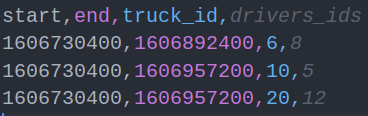
\includegraphics[width=0.8\linewidth]{photo/schedule_table}
	\caption{Пример таблицы графика поставок}
	\label{schedule_table}
\end{figure}

\newpage

Для запросов определены следующие столбцы:
\begin{itemize}
	\item destination -- код конечного пункта (int);
	\item departure\_date -- дата отправки в формате дд.мм.гггг чч:мм (string);
	\item cargo\_weight -- масса груза (float);
	\item truck\_brand -- код предпочитаемой марки грузовика (int).
\end{itemize}

Пример запроса указан на рис. \ref{request_table}.

\begin{figure}[hpt!]
	\centering
	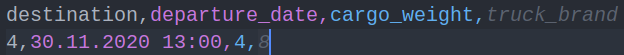
\includegraphics[width=0.8\linewidth]{photo/request_table}
	\caption{Пример запроса}
	\label{request_table}
\end{figure}

Для хранения пароля для доступа к консоли администратора используется обычный текстовый файл, содержащий единственную строку: хэш сумма заданного пароля.

Пример файла с хэшем пароля указан на рис. \ref{hash_example}.

\begin{figure}[hpt!]
	\centering
	
\includegraphics[width=0.8\linewidth]{photo/hash_example}
	\caption{Пример файла с хэшем пароля}
	\label{hash_example}
\end{figure}
	
	\section{Внутренние форматы хранения данных}
\setcounter{figure}{0}

% The 3-Clause BSD License

В данной работе используется комбинация из различных структур данных, 
объединённых в единую систему.
Полная схема структур и их связей представленна на рис. \ref{overall_data_structure}

\begin{figure}[hpt!]
    \centering
    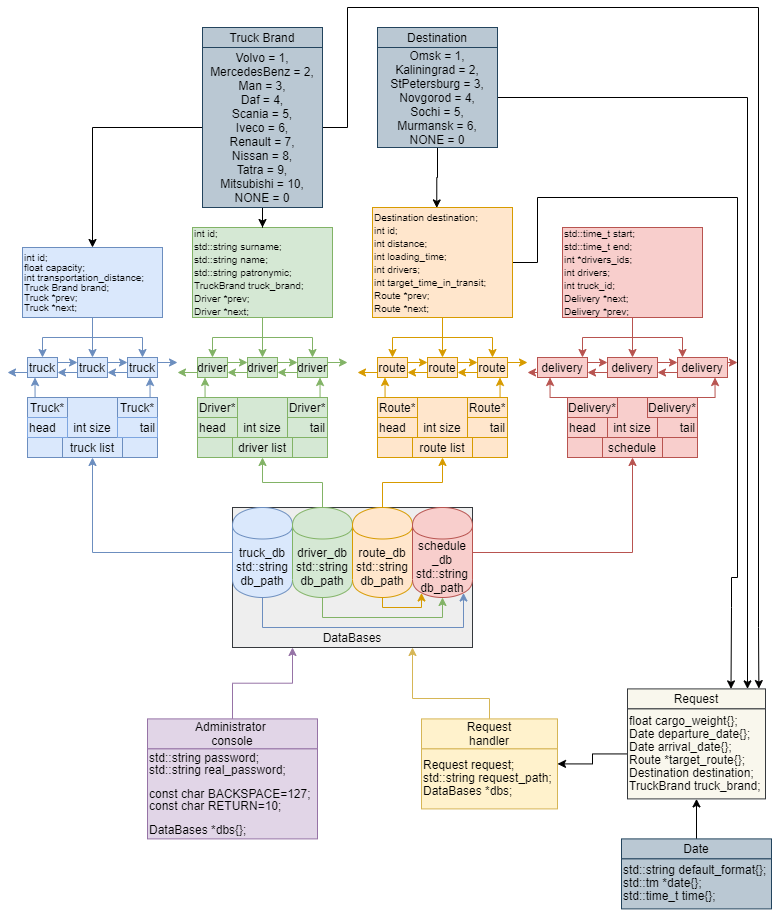
\includegraphics[width=1\linewidth]{photo/overall_data_structure}
    \caption{Обзорная диаграмма структур данных программы}
    \label{overall_data_structure}
\end{figure}

\newpage

\subsection{Структура данных двусвязный список}

В работе предпологается использование структуры данных "список".
Список --- структура данных, состоящая из элементов, 
содержащих помимо собственных данных ссылки на 
следующий и/или предыдущий элемент списка \cite{list_defenition}.

Для работы был вабран вариант с двунаправленым списком, 
где каждый узел имеет указатель на следующий и на предыдущий элементы.
Схема двунаправленного списка показана на рис. \ref{list_schema}.

\begin{figure}[hpt!]
    \centering
    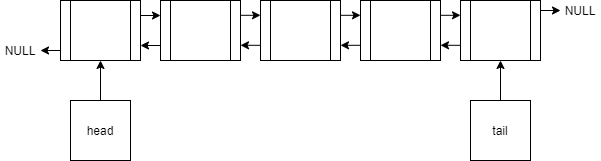
\includegraphics[width=1\linewidth]{photo/list_schema}
    \caption{Схема структуры данных двусвязный список}
    \label{list_schema}
\end{figure}

\subsection{TruckBrand}

Структурой данных \textbf{перечисление} представленны марки грузовиков.
Здесь содержаться все возможные значения марок грузовиков транспортной компании. 

Схема представлена на рис. \ref{truck_brand}

% рисунок

\subsection{Destination}


Возможные маршруты поставки содержаться в структуре данных  \textbf{перечисление}.
Здесь содержаться все возможные значения маршрутов транспортной компании. 

Схема представлена на рис. \ref{destination}

% рисунок

\subsection{Truck}

Представление грузовика в памяти программы выполнено в виде структуры Truck со следующими полями:

\begin{itemize}
    \item 1
\end{itemize}

Схема на рис. \ref{truck}.

% рисунок

\subsection{TruckList}

Для управления списком грузовиков используется структура TruckList со следующими полями:

\begin{itemize}
    \item 1
\end{itemize}

Структура так же содержит методы для управления списком.

Схема на рис. \ref{truck_list}.

% рисунок

\subsection{TruckDataBase}

Для управления базой данных грузовиков, 
её загрузки и обновления, 
используется структура TruckDataBase со следующими полями: 

\begin{itemize}
    \item 1
\end{itemize}

Структура так же содержит методы для управления базой данных.

Схема на рис. \ref{truck_db}.

% рисунок

\subsection{Route}

Представление маршрута в памяти программы выполнено в виде структуры Route со следующими полями:

\begin{itemize}
    \item 1
\end{itemize}

Схема на рис. \ref{route}.

% рисунок

\subsection{RouteList}

Для управления списком маршрутов используется структура RouteList со следующими полями:

\begin{itemize}
    \item 1
\end{itemize}

Структура так же содержит методы для управления списком.

Схема на рис. \ref{route_list}.

% рисунок

\subsection{RouteDataBase}

Для управления базой данных маршрутов, 
её загрузки и обновления, 
используется структура RouteDataBase со следующими полями: 

\begin{itemize}
    \item 1
\end{itemize}

Структура так же содержит методы для управления базой данных.

Схема на рис. \ref{route_db}.

% рисунок

\subsection{Driver}

Представление водителя в памяти программы выполнено в виде структуры Driver со следующими полями:

\begin{itemize}
    \item 1
\end{itemize}

Схема на рис. \ref{driver}.

% рисунок

\subsection{DriverList}

Для управления списком водителей используется структура DriverList со следующими полями:

\begin{itemize}
    \item 1
\end{itemize}

Структура так же содержит методы для управления списком.

Схема на рис. \ref{driver_list}.

% рисунок

\subsection{DriverDataBase}

Для управления базой данных водителей, 
её загрузки и обновления, 
используется структура DriverDataBase со следующими полями: 

\begin{itemize}
    \item 1
\end{itemize}

Структура так же содержит методы для управления базой данных.

Схема на рис. \ref{driver_db}.

% рисунок

\subsection{Delivery}

Представление поставки в памяти программы выполнено в виде структуры Delivery со следующими полями:

\begin{itemize}
    \item 1
\end{itemize}

Схема на рис. \ref{delivery}.

% рисунок

\subsection{Schedule}

Для управления списком поставок используется структура Schedule со следующими полями:

\begin{itemize}
    \item 1
\end{itemize}

Структура так же содержит методы для управления списком.

Схема на рис. \ref{schedule}.

% рисунок

\subsection{ScheduleDataBase}

Для управления базой данных поставок, 
её загрузки и обновления, 
используется структура DriverDataBase со следующими полями: 

\begin{itemize}
    \item 1
\end{itemize}

Структура так же содержит методы для управления базой данных.

Схема на рис. \ref{schedule_db}.

% рисунок

\subsection{DataBases}
\subsection{AdministratorConsole}
\subsection{Date}
\subsection{Request}
\subsection{RequestHandler}

	
	\section{Описание пользовательских функций}

Все функции и модули, реализованные в ходе выполнения данной курсовой работы, представленны в таблице \ref{funcsnmodules}.

\begin{table}[h!]
	\caption{Описание пользовательских функций и модулей программы}
	\label{funcsnmodules}
	\begin{tabular}{|p{2.5cm}|p{2.5cm}|p{2.5cm}|p{2.5cm}|p{2.5cm}|}
		\hline
		Имя модуля & Имя функции & Назначение & Параметры функции & Возращаемое \nl значение функции \\
		\hline
		truck\_brand.h & str & Вывод марки грузовика в виде строки & TruckBrand truck\_brand & std::string\\
		\hline
	\end{tabular} 
\end{table}
	
	Программа разделена на два интерфейса: пользовательский, для получения и обработки запросов, и администраторский, для редактирования и просмотра баз данных.
	
	\section{Алгоритм программы}

\subsection{main}

\begin{lstlisting}
    int main(int argc, char *argv[])
\end{lstlisting}

\begin{itemize}
    \item \verb|DataBases dbs{};|
    \item Если \verb|argc == 1|
    \begin{itemize}
        \item \verb|AdministratorConsole ac{&dbs};|
        \item \verb|return ac.Run();|
    \end{itemize}
    \item Если \verb|argc == 2|
    \begin{itemize}
        \item \verb|RequestHandler rh{argv[1], &dbs};|
        \item \verb|return rh.Run();|
    \end{itemize}
    \item \verb|std::cerr << "Unexpected arguments count\n";|
    \item \verb|return 255;|
\end{itemize}

\subsection{Модуль date.h}


\subsubsection{Date}

\underline{Назначение:} Конструктор для инициализации объекта структуры

\underline{Параметры:} \verb|-|

\underline{Возвращаемое значение:} \verb|Date|


\subsubsection{Date}

\underline{Назначение:} Конструктор для инициализации объекта структуры

\underline{Параметры:} \verb|std::time_t time_to_set|

\underline{Возвращаемое значение:} \verb|Date|


\subsubsection{Date}

\underline{Назначение:} Конструктор для инициализации объекта структуры

\underline{Параметры:} \verb|const std::string &date_str, const std::string &format = ""|

\underline{Возвращаемое значение:} \verb|Date|


\subsubsection{SetFromString}

\underline{Назначение:} Задание даты из строки

\underline{Параметры:} \verb|const std::string &date_str, const std::string &format = ""|

\underline{Возвращаемое значение:} \verb|void|


\subsubsection{SetFromTime}

\underline{Назначение:} Задание даты из времени

\underline{Параметры:} \verb|time_t time_to_set|

\underline{Возвращаемое значение:} \verb|void|


\subsubsection{String}

\underline{Назначение:} Получение стокового представления даты

\underline{Параметры:} \verb|-|

\underline{Возвращаемое значение:} \verb|std::string|


\subsubsection{\_init}

\underline{Назначение:} Инициализация объекта структуры

\underline{Параметры:} \verb|-|

\underline{Возвращаемое значение:} \verb|void|


\subsection{Модуль destination.h}


\subsubsection{str}

\underline{Назначение:} Получение строкового представления точки назначения

\underline{Параметры:} \verb|Destination destination|

\underline{Возвращаемое значение:} \verb|std::string|


\subsection{Модуль schedule.h}


\subsubsection{Get}

\underline{Назначение:} Получение элемента списка

\underline{Параметры:} \verb|int index|

\underline{Возвращаемое значение:} \verb|Delivery *|


\subsubsection{Add}

\underline{Назначение:} Добавление элемента в список

\underline{Параметры:} \verb|const Delivery &delivery|

\underline{Возвращаемое значение:} \verb|Delivery *|


\subsubsection{Delete}

\underline{Назначение:} Удаление элемента из списка

\underline{Параметры:} \verb|int index|

\underline{Возвращаемое значение:} \verb|void|


\subsubsection{Free}

\underline{Назначение:} Очистка списка

\underline{Параметры:} \verb|-|

\underline{Возвращаемое значение:} \verb|void|


\subsubsection{\_check\_index}

\underline{Назначение:} Проверка полученного индекса

\underline{Параметры:} \verb|const int &index|

\underline{Возвращаемое значение:} \verb|void|


\subsection{Модуль administrator\_console.h}


\subsubsection{AdministratorConsole}

\underline{Назначение:} Конструктор для инициализации объекта структуры

\underline{Параметры:} \verb|DataBases *data_bases|

\underline{Возвращаемое значение:} \verb|AdministratorConsole|


\subsubsection{Run}

\underline{Назначение:} Запуск консоли администратора

\underline{Параметры:} \verb|-|

\underline{Возвращаемое значение:} \verb|int|


\subsubsection{\_loadRealPassword}

\underline{Назначение:} Загрузка хэша пароля из файла

\underline{Параметры:} \verb|-|

\underline{Возвращаемое значение:} \verb|void|


\subsubsection{\_uploadPassword}

\underline{Назначение:} Загрузка хэша пароля в файл

\underline{Параметры:} \verb|-|

\underline{Возвращаемое значение:} \verb|void|


\subsubsection{\_getch}

\underline{Назначение:} 
Получение символа с клавиатуры без его вывода на экран

\underline{Параметры:} \verb|-|

\underline{Возвращаемое значение:} \verb|int|


\subsubsection{\_inputPassword}

\underline{Назначение:} Ввод пароля

\underline{Параметры:} 
\verb|const std::string &prompt, bool show_asterisk=true|

\underline{Возвращаемое значение:} \verb|void|


\subsubsection{\_verifyPassword}

\underline{Назначение:} Сравнение хэша пароля с заданным

\underline{Параметры:} \verb|-|

\underline{Возвращаемое значение:} \verb|bool|


\subsubsection{\_mainMenu}

\underline{Назначение:} Главное меню

\underline{Параметры:} \verb|-|

\underline{Возвращаемое значение:} \verb|int|


\subsubsection{\_truckMenu}

\underline{Назначение:} Меню для работы с базой данных грузовиков

\underline{Параметры:} \verb|-|

\underline{Возвращаемое значение:} \verb|void|


\subsubsection{\_driverMenu}

\underline{Назначение:} Меню для работы с базой данных водителей

\underline{Параметры:} \verb|-|

\underline{Возвращаемое значение:} \verb|void|


\subsubsection{\_routeMenu}

\underline{Назначение:} Меню для работы с базой данных маршрутов

\underline{Параметры:} \verb|-|

\underline{Возвращаемое значение:} \verb|void|


\subsubsection{\_changePassword}

\underline{Назначение:} Смена установленного пароля на новый

\underline{Параметры:} \verb|-|

\underline{Возвращаемое значение:} \verb|void|


\subsection{Модуль truck\_db}

\subsubsection{TruckDataBase}

\begin{lstlisting}
    TruckDataBase(ScheduleDataBase *schedule_p, const std::string &db_path_ = "../dbs/truckdb.csv");
\end{lstlisting}

\begin{itemize}
    \item \verb|schedule = schedule_p;|
    \item \verb|db_path = db_path_;|
    \item \verb|_loadDataBase();|
\end{itemize}

\subsubsection{PrintAll}

\begin{lstlisting}
    void PrintAll() const;
\end{lstlisting}

\begin{itemize}
    \item \verb|std::cout << std::left|\\
    \verb|<< std::setw(4)  << "id "|\\
    \verb|<< std::setw(14) << "brand "|\\
    \verb|<< std::setw(10)  << "capacity "|\\
    \verb|<< std::setw(5)  << "transportation_distance\n";|
    \item Цикл по \verb|i| от \verb|0| до \verb|list.size| 
        \begin{itemize}
            \item \verb|Print(i);|
        \end{itemize}
\end{itemize}

\subsubsection{Print}

\begin{lstlisting}
    void Print(int index) const;
\end{lstlisting}

\begin{itemize}
    \item \verb|list._check_index(index);|
    \item \verb|auto p = list.Get(index);|
    \item \verb|std::cout << std::left|
          \verb|<< std::setw(3)  << p-> id << " "|\\
          \verb|<< std::setw(13) << str(p->brand) << " "|\\
          \verb|<< std::setw(9)  << p->capacity << " "|\\
          \verb|<< std::setw(5)  << p->transportation_distance << "\n";|
\end{itemize}

\subsubsection{Find}

\begin{lstlisting}
    Truck *Find(Request *request) const;
\end{lstlisting}

\begin{itemize}
    \item \verb|Truck *pTruck = list.head;|
    \item Пока \verb|pTruck|
    \begin{itemize}
        \item Если \verb|(|\\
        \verb|(pTruck->brand != request->truck_brand) |||\\
        \verb|(pTruck->capacity < request->cargo_weight) |||\\ 
        \verb|(pTruck->transportation_distance < request->target_route->distance) |||\\
        \verb|(!schedule->IsFree(pTruck, request))|\\
        \verb|)|
            \begin{itemize}
                \item \verb|pTruck = pTruck->next;|
                \item \verb|continue;|
            \end{itemize}
        \item \verb|return pTruck;|
    \end{itemize}
    \item \verb|return nullptr;|
\end{itemize}

\subsubsection{Edit}

\begin{lstlisting}
    void Edit(int index);
\end{lstlisting}

\begin{itemize}
    \item \verb|list._check_index(index);|
    \item \verb|Truck *target_element = list.Get(index);|
    \item Пока \verb|true|
        \begin{itemize}
            \item \verb|std::cout << "------------------------\n";|
            \item \verb|Print(index);|
            \item \verb|std::cout << "------------------------\n";|
            \item \verb|std::cout << "Choose filed:\n";|
            \item \verb|std::cout << "1 brand" << "\n";|
            \item \verb|std::cout << "2 capacity" << "\n";|
            \item \verb|std::cout << "3 distance" << "\n";|
            \item \verb|std::cout << "0 Finish edit" << "\n";|
            \item \verb|int option = InputInt("Input: ");|
            \item Смотрим на \verb|option|
            \begin{itemize}
                \item Если \verb|1:|
                \item \verb|    target_element->brand = InputTB("New value: ");|
                \item \verb|    break;|
                \item Если \verb|2:|
                \item \verb|    target_element->capacity = InputInt("New value: ");|
                \item \verb|    break;|
                \item Если \verb|3:|
                \item \verb|    target_element->transportation_distance = InputInt("New value: ");|
                \item \verb|    break;|
                \item Если \verb|0: _updateDbFile(); return;|
                \item По умолчанию \verb|: std::cout << "\nIncorrect input\n\n";|
            \end{itemize}
        \end{itemize}
\end{itemize}

\subsubsection{Add}

\begin{lstlisting}
    void Add();
\end{lstlisting}

\begin{itemize}
    \item \verb|Truck new_element;|
    \item \verb|new_element.id = list.Get(list.size-1)->id + 1;|
    \item \verb|new_element.brand = InputTB("brand: ");|
    \item \verb|new_element.capacity = InputInt("capacity: ");|
    \item \verb|new_element.transportation_distance = InputInt("transportation distance: ");|
    \item \verb|list.Add(new_element);|
    \item \verb|_updateDbFile();|
\end{itemize}

\subsubsection{Delete}

\begin{lstlisting}
    void Delete(int index);
\end{lstlisting}

\begin{itemize}
    \item \verb|list.Delete(index);|
    \item Цикл по \verb|i| от \verb|index| до \verb|list.size| 
    \begin{itemize}
        \item \verb|list.Get(i)->id = i;|
    \end{itemize}
    \item \verb|_updateDbFile();|
\end{itemize}

\subsubsection{Exit}

\begin{lstlisting}
    void Exit();
\end{lstlisting}

\begin{itemize}
    \item \verb|list.Free();|
\end{itemize}

\subsubsection{\_loadDataBase}

\begin{lstlisting}
    void _loadDataBase();
\end{lstlisting}

\begin{itemize}
    \item \verb|Truck truck{};|
    \item \verb|io::CSVReader<4> in(db_path);|
    \item \verb|in.read_header(io::ignore_extra_column, "id", "brand", "capacity", "transportation_distance");|
    \item \verb|int brand_code;|
    \item Пока \verb|in.read_row(truck.id, brand_code, truck.capacity, truck.transportation_distance)|
        \begin{itemize}
            \item \verb|truck.brand = static_cast<TruckBrand>(brand_code);|
            \item \verb|list.Add(truck);|
        \end{itemize}
\end{itemize}

\subsubsection{\_updateDbFile}

\begin{lstlisting}
    void _updateDbFile() const;
\end{lstlisting}

\begin{itemize}
    \item \verb|std::ofstream fout(db_path, std::ios_base::trunc);|
    \item \verb|fout << "id,brand,capacity,transportation_distance\n";|
    \item \verb|Truck *p = list.head;|
    \item Пока \verb|p|
        \begin{itemize}
            \item 
            \verb|fout << p->id << ","|\\
            \verb|     << static_cast<int>(p->brand) << ","|\\
            \verb|     << p->capacity << ","|\\
            \verb|     << p->transportation_distance;|
            \item \verb|fout << "\n";|
            \item \verb|p = p->next;|
        \end{itemize}
\end{itemize}


\subsection{Модуль route.h}


\subsubsection{Route}

\underline{Назначение:} Конструктор для инициализации объекта структуры

\underline{Параметры:} \verb|-|

\underline{Возвращаемое значение:} \verb|Route|


\subsubsection{Route}

\underline{Назначение:} Конструктор для инициализации объекта структуры

\underline{Параметры:} \verb|const Route &route|

\underline{Возвращаемое значение:} \verb|Route|


\subsection{Модуль schedule\_db}

\subsubsection{ScheduleDataBase}

\begin{lstlisting}
    ScheduleDataBase(const std::string &db_path_ = "../dbs/scheduledb.csv");
\end{lstlisting}

\begin{itemize}
    \item \verb|db_path = db_path_;|
    \item \verb|_loadDataBase();|
\end{itemize}

\subsubsection{PrintAll}

\begin{lstlisting}
    void PrintAll() const;
\end{lstlisting}

\begin{itemize}
    \item Цикл по \verb|i| от \verb|0| до \verb|list.size| 
        \begin{itemize}
            \item \verb|Print(i);|
        \end{itemize}
\end{itemize}

\subsubsection{Print}

\begin{lstlisting}
    void Print(int index) const;
\end{lstlisting}

\begin{itemize}
    \item \verb|list._check_index(index);|
    \item \verb|auto p = list.Get(index);|
    \item \verb|std::cout << p->start << " "|\\
          \verb|<< p->end << " "|\\
          \verb|<< p->truck_id << " ";|
    \item Цикл по \verb|i| от \verb|0| до \verb|p->drivers| 
        \begin{itemize}
            \item \verb|std::cout << p->drivers_ids[i] << ";";|
        \end{itemize}
    \item \verb|std::cout << "\n";|
\end{itemize}

\subsubsection{IsFree}

\begin{lstlisting}
    bool IsFree(Truck *truck, Request *request) const;
\end{lstlisting}

\begin{itemize}
    \item \verb|Delivery *pDelivery = list.head;|
    \item Пока \verb|pDelivery|
        \begin{itemize}
            \item Если \verb|pDelivery->truck_id == truck->id|
            \begin{itemize}
                \item Если \verb|_isIntersection(pDelivery, request)|
                \item \verb|    return false;|
            \end{itemize}
            \item \verb|pDelivery = pDelivery->next;|
        \end{itemize}
    \item \verb|return true;|
\end{itemize}

\subsubsection{IsFree}

\begin{lstlisting}
    bool IsFree(Driver *driver, Request *request) const;
\end{lstlisting}

\begin{itemize}
    \item \verb|Delivery *pDelivery = list.head;|
    \item Пока \verb|pDelivery|
        \begin{itemize}
            \item Цикл по \verb|i| от \verb|0| до \verb|pDelivery->drivers| 
            \begin{itemize}
                \item Если \verb|pDelivery->drivers_ids[i] == driver->id|
                \begin{itemize}
                    \item Если \verb|_isIntersection(pDelivery, request)|
                    \item \verb|    return false;|
                \end{itemize}
            \end{itemize}
            \item \verb|pDelivery = pDelivery->next;|
        \end{itemize}
    \item \verb|return true;|
\end{itemize}

\subsubsection{Update}

\begin{lstlisting}
    void Update(Date *current_date);
\end{lstlisting}

\begin{itemize}
    \item \verb|Delivery *pDelivery = list.head;|
    \item \verb|int index = 0;|
    \item Пока \verb|pDelivery|
        \begin{itemize}
            \item \verb|Delivery *next = pDelivery->next;|
            \item Если \verb|pDelivery->end < date->time|
            \item \verb|    list.Delete(index);|
            \item Иначе
            \item \verb|    ++index;|
            \item \verb|pDelivery = next;|
        \end{itemize}
    \item \verb|_updateDbFile();|
\end{itemize}

\subsubsection{Add}

\begin{lstlisting}
    void Add(Delivery *delivery);
\end{lstlisting}

\begin{itemize}
    \item \verb|list.Add(*delivery);|
    \item \verb|_updateDbFile();|
\end{itemize}

\subsubsection{Exit}

\begin{lstlisting}
    lst
\end{lstlisting}

\begin{itemize}
    \item \verb||
\end{itemize}

\subsubsection{\_loadDataBase}

\begin{lstlisting}
    lst
\end{lstlisting}

\begin{itemize}
    \item \verb||
\end{itemize}

\subsubsection{\_updateDbFile}

\begin{lstlisting}
    lst
\end{lstlisting}

\begin{itemize}
    \item \verb||
\end{itemize}

\subsubsection{\_parseDriversIdsStr}

\begin{lstlisting}
    lst
\end{lstlisting}

\begin{itemize}
    \item \verb||
\end{itemize}

\subsubsection{\_isIntersection}

\begin{lstlisting}
    lst
\end{lstlisting}

\begin{itemize}
    \item \verb||
\end{itemize}


\subsection{Модуль route\_db}

\subsubsection{RouteDataBase}

\begin{lstlisting}
    RouteDataBase(const std::string &db_path_ = "../dbs/routedb.csv");
\end{lstlisting}

\begin{itemize}
    \item \verb|db_path = db_path_;|
    \item \verb|_loadDataBase();|
\end{itemize}

\subsubsection{PrintAll}

\begin{lstlisting}
    void PrintAll() const;
\end{lstlisting}

\begin{itemize}
    \item \verb|std::cout << std::left|\\
          \verb|<< std::setw(4)   << "id "|\\
          \verb|<< std::setw(15)  << "destination "|\\
          \verb|<< std::setw(15)  << "distance "|\\
          \verb|<< std::setw(15)  << "loading_time "|\\
          \verb|<< std::setw(15)  << "drivers "|\\
          \verb|<< std::setw(15)  << "target_time_in_transit\n";|
    \item Цикл по \verb|i| от \verb|0| до \verb|list.size| 
        \begin{itemize}
            \item \verb|Print(i);|
        \end{itemize}
    \item \verb||
\end{itemize}

\subsubsection{Print}

\begin{lstlisting}
    void Print(int index) const;
\end{lstlisting}

\begin{itemize}
    \item \verb|list._check_index(index);|
    \item \verb|auto p = list.Get(index);|
    \item \verb|std::cout << std::left|\\
          \verb|<< std::setw(3)  << p->id << " "|\\
          \verb|<< std::setw(14) << str(p->destination) << " "|\\
          \verb|<< std::setw(14)  << p->distance << " "|\\
          \verb|<< std::setw(14)  << p->loading_time << " "|\\
          \verb|<< std::setw(14)  << p->drivers << " "|\\
          \verb|<< std::setw(15)  << p->target_time_in_transit << "\n";|
\end{itemize}

\subsubsection{Find}

\begin{lstlisting}
    Route *Find(Destination destination) const;
\end{lstlisting}

\begin{itemize}
    \item Цикл по \verb|i| от \verb|0| до \verb|list.size| 
        \begin{itemize}
            \item \verb|Route *current_route = list.Get(i);|
            \item Если \verb|current_route->destination == destination|
            \item \verb|    return current_route;|
        \end{itemize}
    \item \verb|return nullptr;|
\end{itemize}

\subsubsection{Edit}

\begin{lstlisting}
    void Edit(int index);
\end{lstlisting}

\begin{itemize}
    \item \verb|list._check_index(index);|
    \item \verb|Route *target_element = list.Get(index);|
    \item Пока \verb|true|
        \begin{itemize}
            \item \verb|std::cout << "------------------------\n";|
            \item \verb|Print(index);|
            \item \verb|std::cout << "------------------------\n";|
            \item \verb|std::cout << "Choose filed:\n";|
            \item \verb|std::cout << "1 destination" << "\n";|
            \item \verb|std::cout << "2 distance" << "\n";|
            \item \verb|std::cout << "3 loading_time" << "\n";|
            \item \verb|std::cout << "4 drivers" << "\n";|
            \item \verb|std::cout << "5 time in transit" << "\n";|
            \item \verb|std::cout << "0 Finish edit" << "\n";|
            \item \verb|int option = InputInt("Input: ");|
            \item Смотрим на \verb|option|
            \begin{itemize}
                \item Если \verb|1:|
                \item \verb|    target_element->destination = InputDest("New value: ");|
                \item \verb|    break;|
                \item Если \verb|2:|
                \item \verb|    target_element->distance = InputInt("New value: ");|
                \item \verb|    break;|
                \item Если \verb|3:|
                \item \verb|    target_element->loading_time = InputInt("New value: ");|
                \item \verb|    break;|
                \item Если \verb|4:|
                \item \verb|    target_element->drivers = InputInt("New value: ");|
                \item \verb|    break;|
                \item Если \verb|5:|
                \item \verb|    target_element->target_time_in_transit = InputInt("New value: ");|
                \item \verb|    break;|
                \item Если \verb|0: _updateDbFile(); return;|
                \item По умолчанию \verb|: std::cout << "\nIncorrect input\n\n";|
            \end{itemize}
        \end{itemize}
\end{itemize}

\subsubsection{Add}

\begin{lstlisting}
    void Add();
\end{lstlisting}

\begin{itemize}
    \item \verb|Route new_element;|
    \item \verb|new_element.id = list.Get(list.size-1)->id + 1;|
    \item \verb|new_element.destination = InputDest("destination: ");|
    \item \verb|new_element.distance = InputInt("distance: ");|
    \item \verb|new_element.loading_time = InputInt("loading_time: ");|
    \item \verb|new_element.drivers = InputInt("drivers: ");|
    \item \verb|new_element.target_time_in_transit = InputInt("time in transit: ");|
    \item \verb|list.Add(new_element);|
    \item \verb|_updateDbFile();|
\end{itemize}

\subsubsection{Delete}

\begin{lstlisting}
    void Delete(int index);
\end{lstlisting}

\begin{itemize}
    \item \verb|list.Delete(index);|
    \item Цикл по \verb|i| от \verb|index| до \verb|list.size| 
    \begin{itemize}
        \item \verb|list.Get(i)->id = i;|
    \end{itemize}
    \item \verb|_updateDbFile();|
\end{itemize}

\subsubsection{Exit}

\begin{lstlisting}
    void Exit();
\end{lstlisting}

\begin{itemize}
    \item \verb|list.Free();|
\end{itemize}

\subsubsection{\_loadDataBase}

\begin{lstlisting}
    void _loadDataBase();
\end{lstlisting}

\begin{itemize}
    \item \verb|Route route{};|
    \item \verb|io::CSVReader<6> in(db_path);|
    \item \verb|in.read_header(io::ignore_extra_column, "id", "destination_code",|
    \verb|"distance", "loading_time", "drivers", "time_in_transit");|
    \item \verb|int destination_code;|
    \item Пока \verb|in.read_row(route.id, destination_code, route.distance,|
               \verb|route.loading_time, route.drivers, route.target_time_in_transit)|
        \begin{itemize}
            \item \verb|route.destination = static_cast<Destination>(destination_code);|
            \item \verb|list.Add(route);|
        \end{itemize}
\end{itemize}

\subsubsection{\_updateDbFile}

\begin{lstlisting}
    void _updateDbFile() const;
\end{lstlisting}

\begin{itemize}
    \item \verb|std::ofstream fout(db_path, std::ios_base::trunc);|
    \item \verb|fout << "id,destination_code,distance,loading_time,drivers,time_in_transit\n";|
    \item \verb|Route *p = list.head;|
    \item Пока \verb|p|
        \begin{itemize}
            \item 
            \verb|fout << p->id << ","|\\
            \verb|     << static_cast<int>(p->destination) << ","|\\
            \verb|     << p->distance << ","|\\
            \verb|     << p->loading_time << ","|\\
            \verb|     << p->drivers << ","|\\
            \verb|     << p->target_time_in_transit;|
            \item \verb|fout << "\n";|
            \item \verb|p = p->next;|
        \end{itemize}
\end{itemize}


\subsection{Модуль input.h}


\subsubsection{InputInt}

\underline{Назначение:} Ввод числа

\underline{Параметры:} \verb|const std::string& message = "Input: ", int l = _min_int, int r = _max_int|

\underline{Возвращаемое значение:} \verb|int|


\subsubsection{InputStr} 

\underline{Назначение:} Ввод строки

\underline{Параметры:} \verb|const std::string& message = "Input: "|

\underline{Возвращаемое значение:} \verb|std::string|


\subsubsection{InputTB}

\underline{Назначение:} Ввод марки грузовика

\underline{Параметры:} \verb|const std::string& message = "Input: "|

\underline{Возвращаемое значение:} \verb|TruckBrand|


\subsubsection{InputDest}

\underline{Назначение:} Ввод точки назначения

\underline{Параметры:} \verb|const std::string& message = "Input: "|

\underline{Возвращаемое значение:} \verb|Destination|


\subsection{Модуль dbs}

\subsubsection{DataBases}

\begin{lstlisting}
    DataBases();
\end{lstlisting}

\begin{itemize}
    \item \verb|schedule_db = ScheduleDataBase();|
    \item \verb|truck_db = TruckDataBase(&schedule_db);|
    \item \verb|driver_db = DriverDataBase(&schedule_db);|
    \item \verb|route_db = RouteDataBase();|
\end{itemize}

\subsubsection{CloseAll}

\begin{lstlisting}
    void CloseAll();
\end{lstlisting}

\begin{itemize}
    \item \verb|schedule_db.Exit();|
    \item \verb|truck_db.Exit();|
    \item \verb|driver_db.Exit();|
    \item \verb|route_db.Exit();|
\end{itemize}


\subsection{Модуль route\_list}

\subsubsection{Get}

\begin{lstlisting}
    lst
\end{lstlisting}

\begin{itemize}
    \item \verb||
\end{itemize}

\subsubsection{Add}

\begin{lstlisting}
    lst
\end{lstlisting}

\begin{itemize}
    \item \verb||
\end{itemize}

\subsubsection{Delete}

\begin{lstlisting}
    lst
\end{lstlisting}

\begin{itemize}
    \item \verb||
\end{itemize}

\subsubsection{Free}

\begin{lstlisting}
    lst
\end{lstlisting}

\begin{itemize}
    \item \verb||
\end{itemize}

\subsubsection{\_check\_index}

\begin{lstlisting}
    lst
\end{lstlisting}

\begin{itemize}
    \item \verb||
\end{itemize}


\subsection{Модуль request\_handler.h}


\subsubsection{RequestHandler}

\underline{Назначение:} Конструктор для инициализации объекта структуры

\underline{Параметры:} \verb|const std::string & request_file_path, DataBases * data_bases|

\underline{Возвращаемое значение:} \verb|RequestHandler|


\subsubsection{Run} 

\underline{Назначение:} Запуск обработчика запроса

\underline{Параметры:} \verb|-|

\underline{Возвращаемое значение:} \verb|int|


\subsubsection{\_loadRequest}

\underline{Назначение:} Загрузка файла с запросом

\underline{Параметры:} \verb|-|

\underline{Возвращаемое значение:} \verb|void|


\subsection{Модуль delivery}

\subsubsection{Delivery}

\begin{lstlisting}
    lst
\end{lstlisting}

\begin{itemize}
    \item \verb||
\end{itemize}

\subsubsection{Delivery}

\begin{lstlisting}
    lst
\end{lstlisting}

\begin{itemize}
    \item \verb||
\end{itemize}

\subsubsection{\_init}

\begin{lstlisting}
    lst
\end{lstlisting}

\begin{itemize}
    \item \verb||
\end{itemize}


\subsection{Модуль truck\_brand}

\subsubsection{str}

\begin{lstlisting}
    lst
\end{lstlisting}

\begin{itemize}
    \item \verb||
\end{itemize}


\subsection{Модуль truck}

\subsubsection{Truck}

\begin{lstlisting}
    lst
\end{lstlisting}

\begin{itemize}
    \item \verb||
\end{itemize}

\subsubsection{Truck}

\begin{lstlisting}
    lst
\end{lstlisting}

\begin{itemize}
    \item \verb||
\end{itemize}


\subsection{Модуль driver.h}


\subsubsection{Driver}

\underline{Назначение:} Конструктор для инициализации объекта структуры

\underline{Параметры:} \verb|-|

\underline{Возвращаемое значение:} \verb|Driver|


\subsubsection{Driver}

\underline{Назначение:} Конструктор для инициализации объекта структуры

\underline{Параметры:} \verb|const Driver &driver|

\underline{Возвращаемое значение:} \verb|Driver|


\subsection{Модуль driver\_db}

\subsubsection{DriverDataBase}

\begin{lstlisting}
    lst
\end{lstlisting}

\begin{itemize}
    \item \verb||
\end{itemize}

\subsubsection{PrintAll}

\begin{lstlisting}
    lst
\end{lstlisting}

\begin{itemize}
    \item \verb||
\end{itemize}

\subsubsection{Print}

\begin{lstlisting}
    lst
\end{lstlisting}

\begin{itemize}
    \item \verb||
\end{itemize}

\subsubsection{Find}

\begin{lstlisting}
    lst
\end{lstlisting}

\begin{itemize}
    \item \verb||
\end{itemize}

\subsubsection{Edit}

\begin{lstlisting}
    lst
\end{lstlisting}

\begin{itemize}
    \item \verb||
\end{itemize}

\subsubsection{Add}

\begin{lstlisting}
    lst
\end{lstlisting}

\begin{itemize}
    \item \verb||
\end{itemize}

\subsubsection{Delete}

\begin{lstlisting}
    lst
\end{lstlisting}

\begin{itemize}
    \item \verb||
\end{itemize}

\subsubsection{Exit}

\begin{lstlisting}
    lst
\end{lstlisting}

\begin{itemize}
    \item \verb||
\end{itemize}

\subsubsection{\_loadDataBase}

\begin{lstlisting}
    lst
\end{lstlisting}

\begin{itemize}
    \item \verb||
\end{itemize}

\subsubsection{\_updateDbFile}

\begin{lstlisting}
    lst
\end{lstlisting}

\begin{itemize}
    \item \verb||
\end{itemize}


\subsection{Модуль driver\_list.h}


\subsubsection{Get}

\underline{Назначение:} Получение элемента списка

\underline{Параметры:} \verb|int index|

\underline{Возвращаемое значение:} \verb|Driver *|


\subsubsection{Add}

\underline{Назначение:} Добавление элемента в список

\underline{Параметры:} \verb|const Driver &driver|

\underline{Возвращаемое значение:} \verb|Driver *|


\subsubsection{Delete}

\underline{Назначение:} Удаление элемента из списка

\underline{Параметры:} \verb|int index|

\underline{Возвращаемое значение:} \verb|void|


\subsubsection{Free}

\underline{Назначение:} Очистка списка

\underline{Параметры:} \verb|-|

\underline{Возвращаемое значение:} \verb|void|


\subsubsection{\_check\_index}

\underline{Назначение:} Проверка полученного индекса

\underline{Параметры:} \verb|const int &index|

\underline{Возвращаемое значение:} \verb|void|


\subsection{Модуль truck\_list}

\subsubsection{Get}

\begin{lstlisting}
    Truck *Get(int index) const;
\end{lstlisting}

\begin{itemize}
    \item \verb|_check_index(index);|
    \item \verb|auto p = head;|
    \item Цикл по \verb|i| от \verb|0| до \verb|index|
        \begin{itemize}
            \item Если \verb|p->next|
            \item \verb|    p = p->next;|
            \item Иначе
            \item \verb|    return nullptr;|
        \end{itemize}
    \item \verb|return p;|
\end{itemize}

\subsubsection{Add}

\begin{lstlisting}
    Truck *Add(const Truck &truck);
\end{lstlisting}

\begin{itemize}
    \item \verb|auto *new_node = new Truck(truck);|
    \item Если \verb|if (size == 0)|
    \begin{itemize}
        \item \verb|head = new_node;|
        \item \verb|tail = new_node;|
        \item \verb|new_node->prev = nullptr;|
        \item \verb|new_node->next = nullptr;|
    \end{itemize}
    \item Иначе
    \begin{itemize}
        \item \verb|new_node->prev = tail;|
        \item \verb|new_node->prev->next = new_node;|
        \item \verb|new_node->next = nullptr;|
        \item \verb|tail = new_node;|
    \end{itemize}
    \item \verb|++size;|
    \item \verb|return new_node;|
\end{itemize}

\subsubsection{Delete}

\begin{lstlisting}
    void Truck(int index);
\end{lstlisting}

\begin{itemize}
    \item \verb|_check_index(index);|
    \item Если \verb|size == 1 && index == 0|
        \begin{itemize}
            \item \verb|Free();|
            \item \verb|return;|
        \end{itemize}
    \item Если \verb|index == 0|
        \begin{itemize}
            \item \verb|Truck *new_head = head->next;|
            \item \verb|delete head;|
            \item \verb|head = new_head;|
            \item \verb|head->prev = nullptr;|
            \item \verb|--size;|
            \item \verb|return;|
        \end{itemize}
    \item Если \verb|index == size - 1|
        \begin{itemize}
            \item \verb|Truck *new_tail = tail->prev;|
            \item \verb|delete tail;|
            \item \verb|tail = new_tail;|
            \item \verb|tail->next = nullptr;|
            \item \verb|--size;|
            \item \verb|return;|
        \end{itemize}
    \item \verb|auto p = Get(index);|
    \item Если \verb|!p|
        \begin{itemize}
            \item \verb|return;|
        \end{itemize}
    \item \verb|p->next->prev = p->prev;|
    \item \verb|p->prev->next = p->next;|
    \item \verb|delete p;|
    \item \verb|--size;|
\end{itemize}

\subsubsection{Free}

\begin{lstlisting}
    void Free();
\end{lstlisting}

\begin{itemize}
    \item \verb|Truck *p = head;|
    \item Пока \verb|p != nullptr|
        \begin{itemize}
            \item \verb|Truck *next = p->next;|
            \item \verb|delete p;|
            \item \verb|p = next;|
        \end{itemize}
    \item \verb|head = nullptr;|
    \item \verb|tail = nullptr;|
    \item \verb|size = 0;|
\end{itemize}

\subsubsection{\_check\_index}

\begin{lstlisting}
    void _check_index(const int &index) const;
\end{lstlisting}

\begin{itemize}
    \item Если \verb|index < 0 |||\verb| index >= size)|
        \begin{itemize}
            \item \verb|std::stringstream message;|
            \item \verb|message << "Index out of range (possible [0-" << size-1 << "], given " << index << ")";|
            \item \verb|throw std::out_of_range(message.str().c_str());|
        \end{itemize}
\end{itemize}
	
	\section{Тестирование программы}

тесты
	
	\section{Выводы}

В результате выполнения данной курсовой работы 
мы закрепили и применили на практике знания, 
полученные в ходе выполнения лабораторных работ. 
Реализованная программа соответствует поставленным задачам 
и безошибочно выполняет свою работу. 
Функционал программы позволяет не только выполнять вычисления, 
но и реализует полноценное взаимодействие с пользователем, 
корректно обрабатывать его запросы и выдавать ему ожидаемый результат. 
Выполнение данной лабораторной работы позволило углубить наши знания 
в технологии программирования многомодульных программ, их реализации 
и отладки.
	
	\addcontentsline{toc}{section}{Список литературы}

\begin{thebibliography}{9} 
    \bibitem{list_defenition}
    Список
    // Викиконспекты
    URL: https://neerc.ifmo.ru/wiki/index.php?title=Список
    (дата обращения: 07.12.2020 г.)
    
    \bibitem{csv}
    CSV
    // Википедия
    URL: https://ru.wikipedia.org/wiki/CSV
    (дата обращения: 14.12.2020 г.)
    
    \bibitem{vscode}
    Visual Studio Code
    // visualstudio
    URL: https://code.visualstudio.com/
    (дата обращения: 16.12.2020 г.)
    
    \bibitem{clion}
    CLion
    // jetbrains
    URL: https://www.jetbrains.com/ru-ru/clion/
    (дата обращения: 16.12.2020 г.)
\end{thebibliography}
	
	\section*{Приложение А. Листинг программного кода}
\addcontentsline{toc}{section}{Приложение А. Листинг программного кода}

\subsection*{administrator\_console.h}
\addcontentsline{toc}{subsection}{administrator\_console.h}
\lstinputlisting[caption=administrator\_console.h]{../src/admin/administrator_console.h}
\newpage

\subsection*{administrator\_console.cpp}
\addcontentsline{toc}{subsection}{administrator\_console.cpp}
\lstinputlisting[caption=administrator\_console.cpp]{../src/admin/administrator_console.cpp}
\newpage

\subsection*{date.h}
\addcontentsline{toc}{subsection}{date.h}
\lstinputlisting[caption=date.h]{../src/common/date.h}
\newpage

\subsection*{date.cpp}
\addcontentsline{toc}{subsection}{date.cpp}
\lstinputlisting[caption=date.cpp]{../src/common/date.cpp}
\newpage

\subsection*{dbs.h}
\addcontentsline{toc}{subsection}{dbs.h}
\lstinputlisting[caption=dbs.h]{../src/common/dbs.h}
\newpage

\subsection*{dbs.cpp}
\addcontentsline{toc}{subsection}{dbs.cpp}
\lstinputlisting[caption=dbs.cpp]{../src/common/dbs.cpp}
\newpage

\subsection*{destination.h}
\addcontentsline{toc}{subsection}{destination.h}
\lstinputlisting[caption=destination.h]{../src/common/destination.h}
\newpage

\subsection*{destination.cpp}
\addcontentsline{toc}{subsection}{destination.cpp}
\lstinputlisting[caption=destination.cpp]{../src/common/destination.cpp}
\newpage

\subsection*{input.h}
\addcontentsline{toc}{subsection}{input.h}
\lstinputlisting[caption=input.h]{../src/common/input.h}
\newpage

\subsection*{input.cpp}
\addcontentsline{toc}{subsection}{input.cpp}
\lstinputlisting[caption=input.cpp]{../src/common/input.cpp}
\newpage

\subsection*{request.h}
\addcontentsline{toc}{subsection}{request.h}
\lstinputlisting[caption=request.h]{../src/common/request.h}
\newpage

\subsection*{truck\_brand.h}
\addcontentsline{toc}{subsection}{truck\_brand.h}
\lstinputlisting[caption=truck\_brand.h]{../src/common/truck_brand.h}
\newpage

\subsection*{truck\_brand.cpp}
\addcontentsline{toc}{subsection}{truck\_brand.cpp}
\lstinputlisting[caption=truck\_brand.cpp]{../src/common/truck_brand.cpp}
\newpage

\subsection*{request\_handler.h}
\addcontentsline{toc}{subsection}{request\_handler.h}
\lstinputlisting[caption=request\_handler.h]{../src/request_handler/request_handler.h}
\newpage

\subsection*{request\_handler.cpp}
\addcontentsline{toc}{subsection}{request\_handler.cpp}
\lstinputlisting[caption=request\_handler.cpp]{../src/request_handler/request_handler.cpp}
\newpage

\subsection*{lib\_truck.h}
\addcontentsline{toc}{subsection}{lib\_truck.h}
\lstinputlisting[caption=lib\_truck.h]{../src/db/truck/lib_truck.h}
\newpage

\subsection*{truck.h}
\addcontentsline{toc}{subsection}{truck.h}
\lstinputlisting[caption=truck.h]{../src/db/truck/truck.h}
\newpage

\subsection*{truck.cpp}
\addcontentsline{toc}{subsection}{truck.cpp}
\lstinputlisting[caption=truck.cpp]{../src/db/truck/truck.cpp}
\newpage

\subsection*{truck\_list.h}
\addcontentsline{toc}{subsection}{truck\_list.h}
\lstinputlisting[caption=truck\_list.h]{../src/db/truck/truck_list.h}
\newpage

\subsection*{truck\_list.cpp}
\addcontentsline{toc}{subsection}{truck\_list.cpp}
\lstinputlisting[caption=truck\_list.cpp]{../src/db/truck/truck_list.cpp}
\newpage

\subsection*{truck\_db.h}
\addcontentsline{toc}{subsection}{truck\_db.h}
\lstinputlisting[caption=truck\_db.h]{../src/db/truck/truck_db.h}
\newpage

\subsection*{truck\_db.cpp}
\addcontentsline{toc}{subsection}{truck\_db.cpp}
\lstinputlisting[caption=truck\_db.cpp]{../src/db/truck/truck_db.cpp}
\newpage

\subsection*{lib\_driver.h}
\addcontentsline{toc}{subsection}{lib\_driver.h}
\lstinputlisting[caption=lib\_driver.h]{../src/db/driver/lib_driver.h}
\newpage

\subsection*{driver.h}
\addcontentsline{toc}{subsection}{driver.h}
\lstinputlisting[caption=driver.h]{../src/db/driver/driver.h}
\newpage

\subsection*{driver.cpp}
\addcontentsline{toc}{subsection}{driver.cpp}
\lstinputlisting[caption=driver.cpp]{../src/db/driver/driver.cpp}
\newpage

\subsection*{driver\_list.h}
\addcontentsline{toc}{subsection}{driver\_list.h}
\lstinputlisting[caption=driver\_list.h]{../src/db/driver/driver_list.h}
\newpage

\subsection*{driver\_list.cpp}
\addcontentsline{toc}{subsection}{driver\_list.cpp}
\lstinputlisting[caption=driver\_list.cpp]{../src/db/driver/driver_list.cpp}
\newpage

\subsection*{driver\_db.h}
\addcontentsline{toc}{subsection}{driver\_db.h}
\lstinputlisting[caption=driver\_db.h]{../src/db/driver/driver_db.h}
\newpage

\subsection*{driver\_db.cpp}
\addcontentsline{toc}{subsection}{driver\_db.cpp}
\lstinputlisting[caption=driver\_db.cpp]{../src/db/driver/driver_db.cpp}
\newpage

\subsection*{lib\_route.h}
\addcontentsline{toc}{subsection}{lib\_route.h}
\lstinputlisting[caption=lib\_route.h]{../src/db/route/lib_route.h}
\newpage

\subsection*{route.h}
\addcontentsline{toc}{subsection}{route.h}
\lstinputlisting[caption=route.h]{../src/db/route/route.h}
\newpage

\subsection*{route.cpp}
\addcontentsline{toc}{subsection}{route.cpp}
\lstinputlisting[caption=route.cpp]{../src/db/route/route.cpp}
\newpage

\subsection*{route\_list.h}
\addcontentsline{toc}{subsection}{route\_list.h}
\lstinputlisting[caption=route\_list.h]{../src/db/route/route_list.h}
\newpage

\subsection*{route\_list.cpp}
\addcontentsline{toc}{subsection}{route\_list.cpp}
\lstinputlisting[caption=route\_list.cpp]{../src/db/route/route_list.cpp}
\newpage

\subsection*{route\_db.h}
\addcontentsline{toc}{subsection}{route\_db.h}
\lstinputlisting[caption=route\_db.h]{../src/db/route/route_db.h}
\newpage

\subsection*{route\_db.cpp}
\addcontentsline{toc}{subsection}{route\_db.cpp}
\lstinputlisting[caption=route\_db.cpp]{../src/db/route/route_db.cpp}
\newpage

\subsection*{lib\_schedule.h}
\addcontentsline{toc}{subsection}{lib\_schedule.h}
\lstinputlisting[caption=lib\_schedule.h]{../src/db/schedule/lib_schedule.h}
\newpage

\subsection*{delivery.h}
\addcontentsline{toc}{subsection}{delivery.h}
\lstinputlisting[caption=delivery.h]{../src/db/schedule/delivery.h}
\newpage

\subsection*{delivery.cpp}
\addcontentsline{toc}{subsection}{delivery.cpp}
\lstinputlisting[caption=delivery.cpp]{../src/db/schedule/delivery.cpp}
\newpage

\subsection*{schedule.h}
\addcontentsline{toc}{subsection}{schedule.h}
\lstinputlisting[caption=schedule.h]{../src/db/schedule/schedule.h}
\newpage

\subsection*{schedule.cpp}
\addcontentsline{toc}{subsection}{schedule.cpp}
\lstinputlisting[caption=schedule.cpp]{../src/db/schedule/schedule.cpp}
\newpage

\subsection*{schedule\_db.h}
\addcontentsline{toc}{subsection}{schedule\_db.h}
\lstinputlisting[caption=schedule\_db.h]{../src/db/schedule/schedule_db.h}
\newpage

\subsection*{schedule\_db.cpp}
\addcontentsline{toc}{subsection}{schedule\_db.cpp}
\lstinputlisting[caption=schedule\_db.cpp]{../src/db/schedule/schedule_db.cpp}
\newpage

\subsection*{libdb.h}
\addcontentsline{toc}{subsection}{libdb.h}
\lstinputlisting[caption=libdb.h]{../src/db/libdb.h}
\newpage

\subsection*{libs.h}
\addcontentsline{toc}{subsection}{libs.h}
\lstinputlisting[caption=libs.h]{../src/libs.h}
\newpage

\subsection*{main.cpp}
\addcontentsline{toc}{subsection}{main.cpp}
\lstinputlisting[caption=main.cpp]{../src/main.cpp}
\newpage
	
\end{document}